\documentclass{article}
\usepackage{lib/setup}
\usepackage{hyperref}
\addbibresource{mybibliography.bib}


%%%%%%%%%%%%%%%%%%%%%%%%%%%%%%%%%%%%%%%%%%%%%%%%%%%%%%%%%%%%%%%%%%%%%%%%%%%%%%%%
%%%%%%%%%%%%%%%%%%%%%%%%%%%%%%%%%%%%%%%%%%%%%%%%%%%%%%%%%%%%%%%%%%%%%%%%%%%%%%%%
%%%%%%%%%%%%%%%%%%%%%%%%%%%%%%%%%%%%%%%%%%%%%%%%%%%%%%%%%%%%%%%%%%%%%%%%%%%%%%%%
% Set up your information
%%%%%%%%%%%%%%%%%%%%%%%%%%%%%%%%%%%%%%%%%%%%%%%%%%%%%%%%%%%%%%%%%%%%%%%%%%%%%%%%
\subtitle{Datapath Verification}
\title{The Shell CPU}
\author{Jonathan Rice Shelley II}
\date{\today}
\headerTitle{Shell CPU}
\subject{Version 1.0}

%%%%%%%%%%%%%%%%%%%%%%%%%%%%%%%%%%%%%%%%%%%%%%%%%%%%%%%%%%%%%%%%%%%%%%%%%%%%%%%%
%%%%%%%%%%%%%%%%%%%%%%%%%%%%%%%%%%%%%%%%%%%%%%%%%%%%%%%%%%%%%%%%%%%%%%%%%%%%%%%%
%%%%%%%%%%%%%%%%%%%%%%%%%%%%%%%%%%%%%%%%%%%%%%%%%%%%%%%%%%%%%%%%%%%%%%%%%%%%%%%%

\newcommand{\stitle}{Component Verification}

% BEGIN DOCUMENT
\begin{document}
\maketitle

\tableofcontents

\newpage

\section{Datapath Verification Overview }
\label{overview}
\begin{par}
	
	\begin{figure}[H]
		\centering
		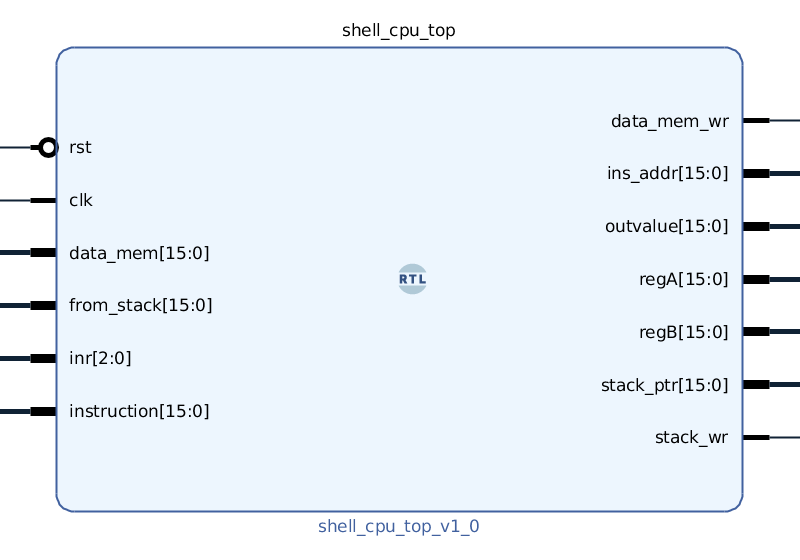
\includegraphics[width=4in]{img/shell_cpu_top.png}
		\caption{Top level CPU design}
		\label{fig:tlcpud}
	\end{figure}
	
	This document details the datapath verification of the Shell CPU. All the datapath components are connected in a top-level component module. The top level Shell CPU module is shown above in Figure \ref{fig:tlcpud}. The VHDL for this module is to long to be listed and can be found with other documentation \href{https://github.com/RiceShelley/ShellCPU}{here}. The top level CPU design can be easily implemented into a larger project like the one shown in Figure \ref{fig:exdesign} to add soft core functionality to a design. 
	
	\begin{figure}[H]
		\centering
		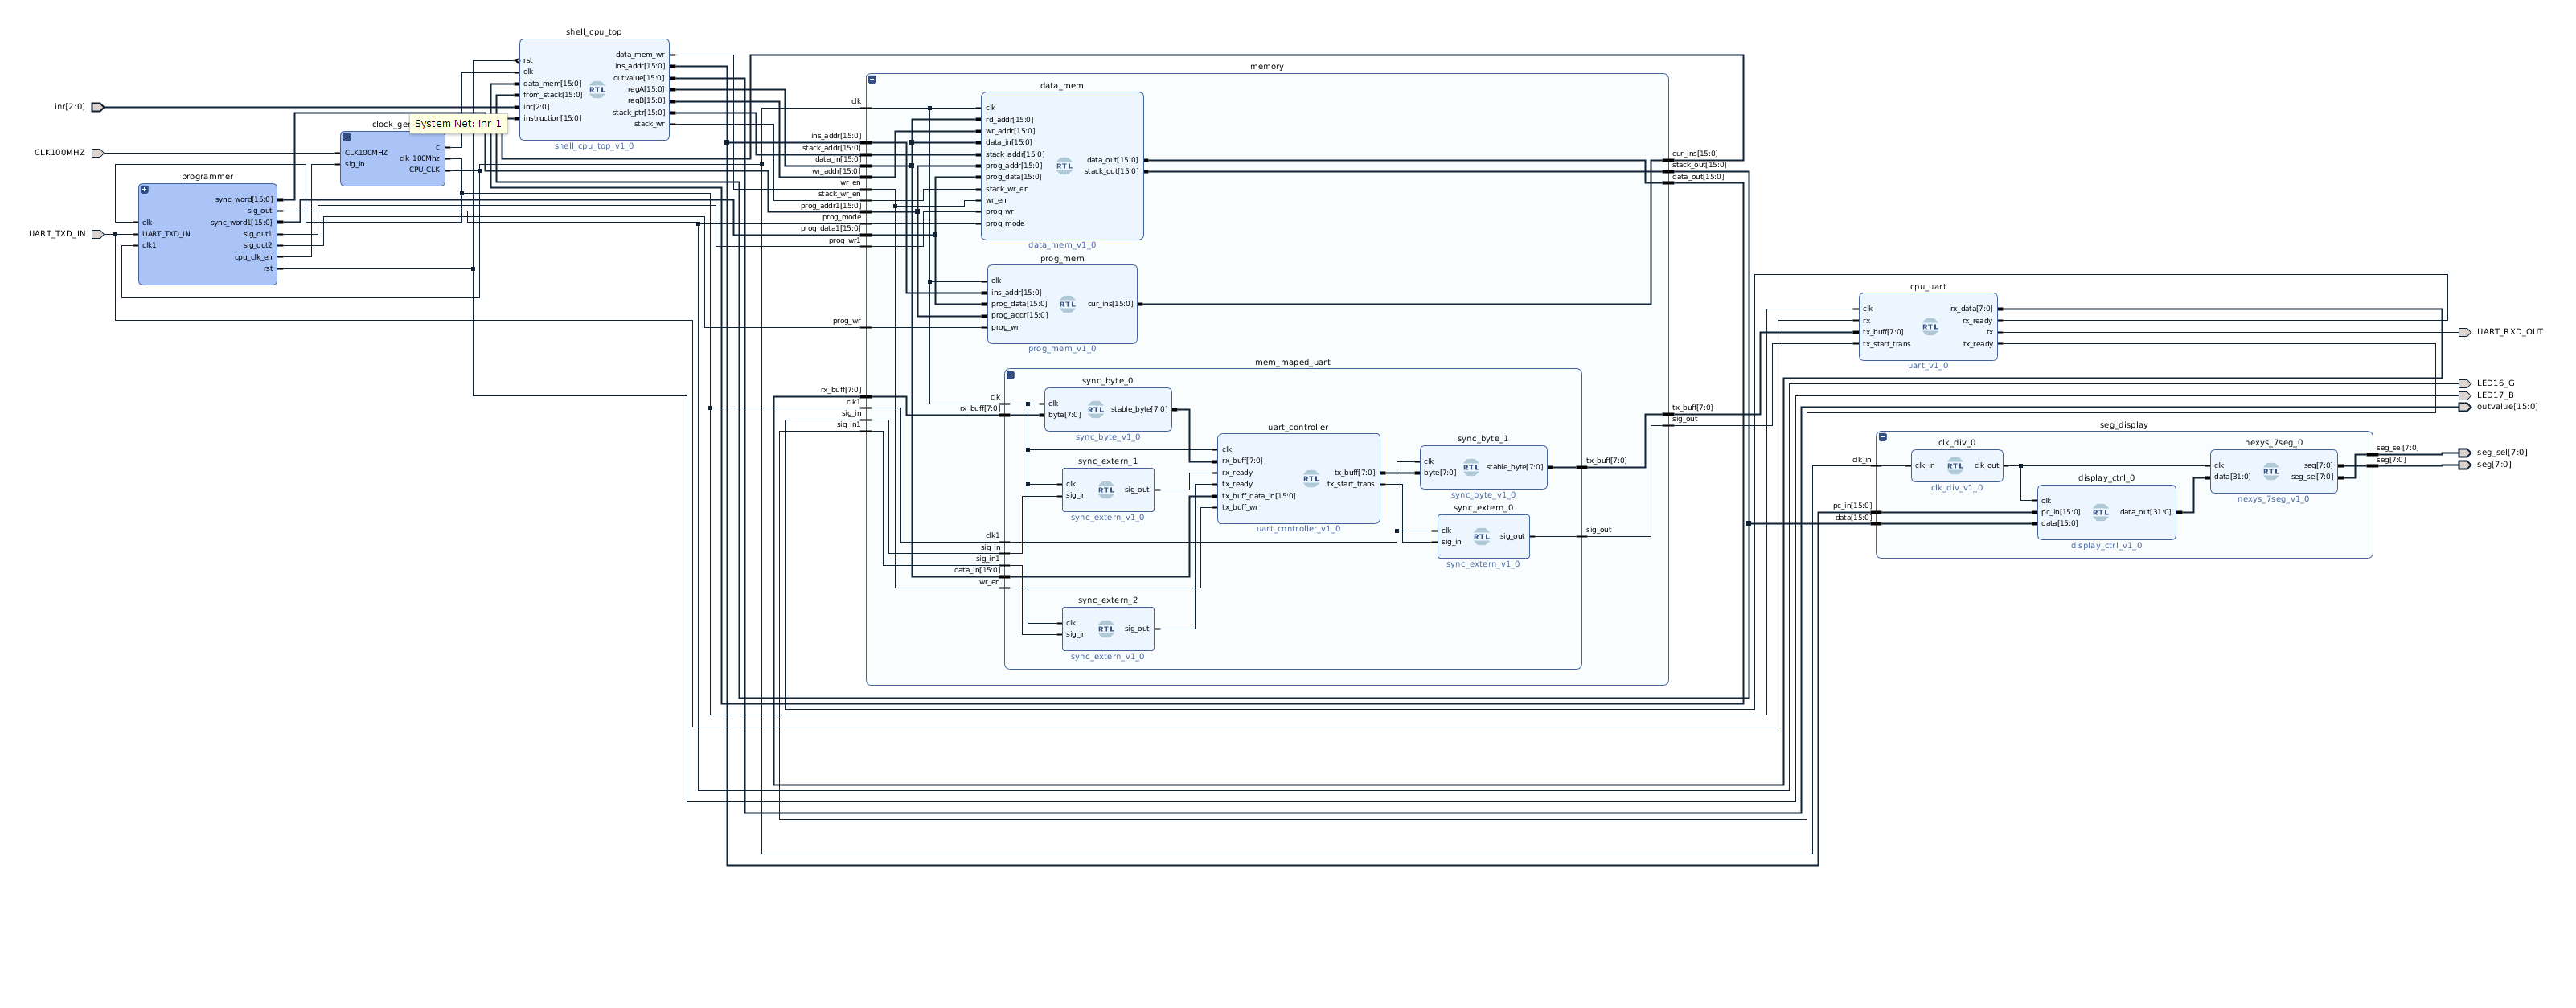
\includegraphics[width=7in]{img/exDesign.png}
		\caption{Example CPU implementation with memory mapped UART hardware / UART programmer}
		\label{fig:exdesign}
	\end{figure}

\end{par}

\newpage

\section{ General Instruction Testing }
\label{CTRL_TEST}

	 A test bench is created to test "general" Shell CPU instructions. General in this case refers to instructions that can be easily tested by viewing the contents of the CPUs register file. Instructions that require a more intensive testing strategy will be verified in a separate section.  
	
	\subsection{Add type RRR instruction verification}
		\vspace{.5cm}
		\begin{center}
			\begin{tabular}{|c|c|}
				\hline 
				\textbf{Instruction} & \textbf{Machine Code} \\ 
				\hline 
				add r3, r1, r2 & 1100000011001010 \\ 
				\hline 
			\end{tabular} 
		\end{center}
		
		\begin{figure}[H]
			\centering
			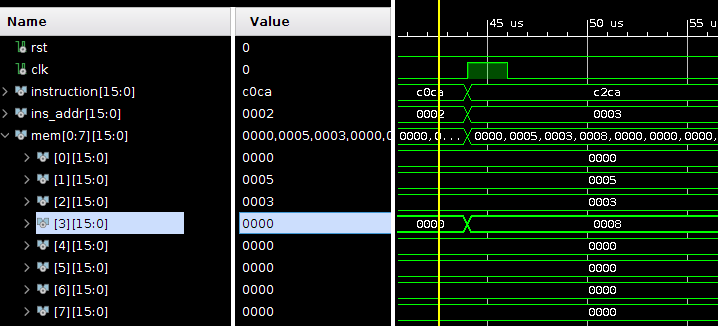
\includegraphics[width=5in]{img/addRRRTest.png}
			\caption{Add RRR instruction simulation}
			\label{fig:addrrrtest}
		\end{figure}
	
		\begin{par}
			A simulation of the Add RRR instruction is shown above in Figure \ref{fig:addrrrtest}. The instruction performs the addition of register one and register two. The sum is stored in register three. In the simulation shown above r1 and r2 can be seen to be five and three respectively. After the positive clock edge the add instruction is executed and eight is seen written to register three. The functionality is verified because the sum of five and three is eight. 
		\end{par}
		\newpage
	
	\subsection{Sub type RRR instruction verification}
		\vspace{.5cm}
		\begin{center}
			\begin{tabular}{|c|c|}
				\hline 
				\textbf{Instruction} & \textbf{Machine Code} \\ 
				\hline 
				sub r3, r1, r2 & 1100001011001010 \\ 
				\hline 
			\end{tabular} 
		\end{center}
		
		\begin{figure}[H]
			\centering
			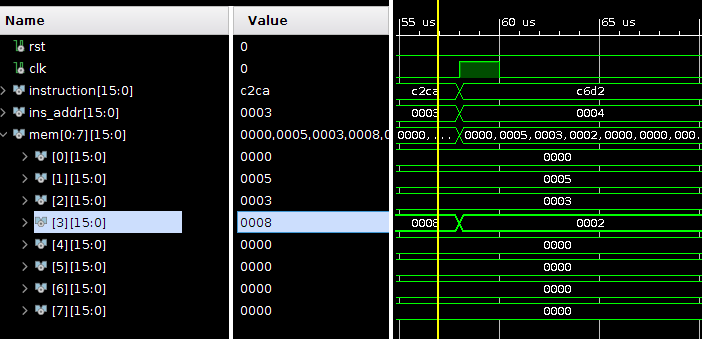
\includegraphics[width=5in]{img/subinstest.png}
			\caption{Sub RRR instruction simulation}
			\label{fig:subrrrtest}
		\end{figure}
		
		\begin{par}
			A simulation of the Sub RRR instruction is shown above in Figure \ref{fig:subrrrtest}. The instruction performs the subtraction of register one and register two. The difference is stored in register three. In the simulation shown above r1 and r2 can be seen to contain five and three respectively. After the positive clock edge the sub instruction is executed and two is seen written to register three. The functionality is verified because the difference of five and three is two. 
		\end{par}
		\newpage

	\subsection{And instruction verification}
		\vspace{.5cm}
		\begin{center}
			\begin{tabular}{|c|c|}
				\hline 
				\textbf{Instruction} & \textbf{Machine Code} \\ 
				\hline 
				and r3, r1, r2 & 1100010011001010 \\ 
				\hline 
			\end{tabular} 
		\end{center}
		
		\begin{figure}[H]
			\centering
			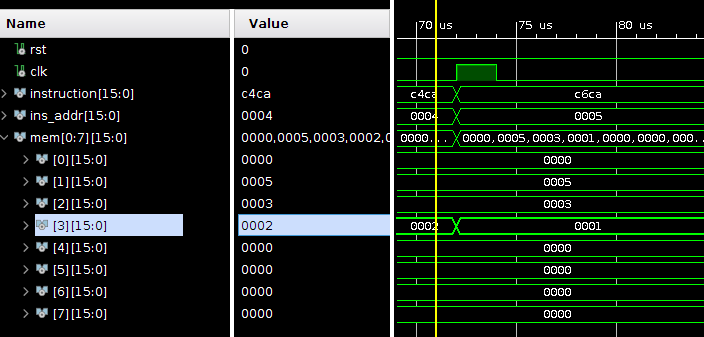
\includegraphics[width=5in]{img/andinstest.png}
			\caption{And instruction simulation}
			\label{fig:andtest}
		\end{figure}
		
		\begin{par}
			A simulation of the and instruction is shown above in Figure \ref{fig:andtest}. The instruction performs the bit wise and of register one and register two. The result is stored in register three. In the simulation shown above r1 and r2 can be seen to contain five and three respectively. After the positive clock edge the and instruction is executed and one is seen written to register three. The functionality is verified because the bit wise and of five and three is one. 
		\end{par}
		\newpage
		
	\subsection{Or instruction verification}
		\vspace{.5cm}
		\begin{center}
			\begin{tabular}{|c|c|}
				\hline 
				\textbf{Instruction} & \textbf{Machine Code} \\ 
				\hline 
				or r3, r1, r2 & 1100011011001010 \\ 
				\hline 
			\end{tabular} 
		\end{center}
		
		\begin{figure}[H]
			\centering
			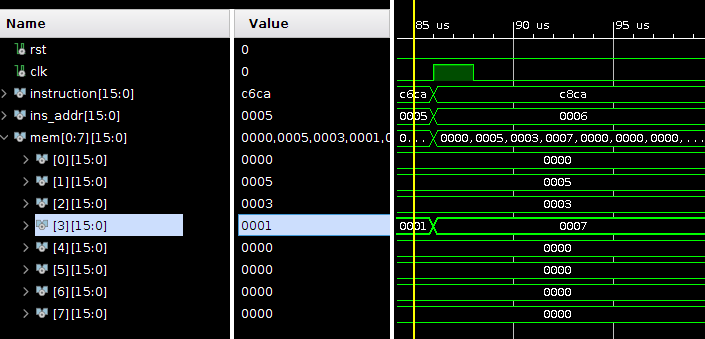
\includegraphics[width=5in]{img/orinstb.png}
			\caption{Or instruction simulation}
			\label{fig:orinstb}
		\end{figure}
		
		\begin{par}
			A simulation of the or instruction is shown above in Figure \ref{fig:orinstb}. The instruction performs the bit wise or of register one and register two. The result is stored in register three. In the simulation shown above r1 and r2 can be seen to contain five and three respectively. After the positive clock edge the or instruction is executed and seven is seen written to register three. The functionality is verified because the bit wise or of five and three is seven. 
		\end{par}
		\newpage
		
	\subsection{Xor instruction verification}
		\vspace{.5cm}
		\begin{center}
			\begin{tabular}{|c|c|}
				\hline 
				\textbf{Instruction} & \textbf{Machine Code} \\ 
				\hline 
				xor r3, r1, r2 & 1100100011001010 \\ 
				\hline 
			\end{tabular} 
		\end{center}
		
		\begin{figure}[H]
			\centering
			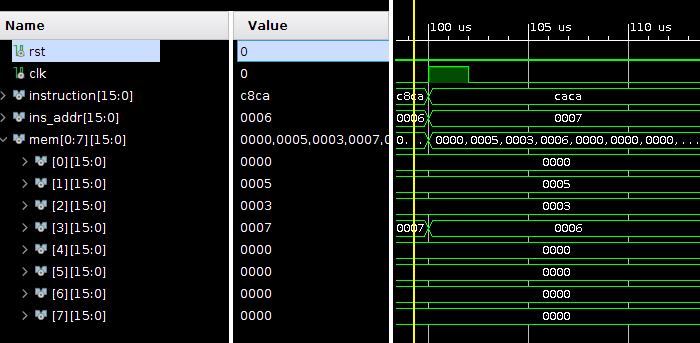
\includegraphics[width=5in]{img/xorinstest.png}
			\caption{Xor instruction simulation}
			\label{fig:xorinstest}
		\end{figure}
		
		\begin{par}
			A simulation of the xor instruction is shown above in Figure \ref{fig:xorinstest}. The instruction performs the bit wise xor of register one and register two. The result is stored in register three. In the simulation shown above r1 and r2 can be seen to contain five and three respectively. After the positive clock edge the xor instruction is executed and six is seen written to register three. The functionality is verified because the bit wise xor of five and three is six. 
		\end{par}
		\newpage

	\subsection{Nand instruction verification}
		\vspace{.5cm}
		\begin{center}
			\begin{tabular}{|c|c|}
				\hline 
				\textbf{Instruction} & \textbf{Machine Code} \\ 
				\hline 
				nand r3, r1, r2 & 1100101011001010 \\ 
				\hline 
			\end{tabular} 
		\end{center}
		
		\begin{figure}[H]
			\centering
			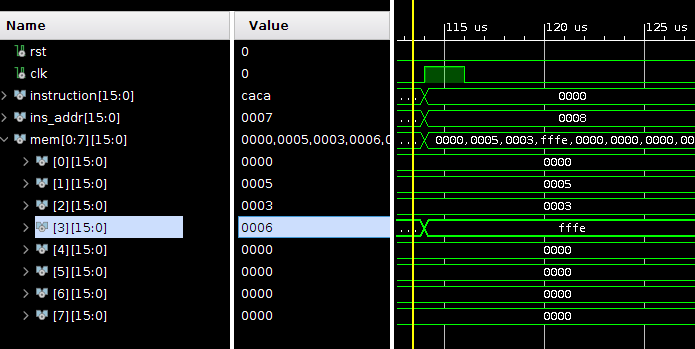
\includegraphics[width=5in]{img/nandinstb.png}
			\caption{Nand instruction simulation}
			\label{fig:nandinstb}
		\end{figure}
		
		\begin{par}
			A simulation of the nand instruction is shown above in Figure \ref{fig:nandinstb}. The instruction performs the bit wise nand of register one and register two. The result is stored in register three. In the simulation shown above r1 and r2 can be seen to contain five and three respectively. After the positive clock edge the nand instruction is executed and 0xfffe is seen written to register three. The functionality is verified because the bit wise nand of five and three is 0xfffe (16-bit hex). 
		\end{par}
		\newpage
		
	\subsection{Asr instruction verification}
		\vspace{.5cm}
		\begin{center}
			\begin{tabular}{|c|c|}
				\hline 
				\textbf{Instruction} & \textbf{Machine Code} \\ 
				\hline 
				asr r3, r1 & 1100110011001000 \\ 
				\hline 
			\end{tabular} 
		\end{center}
		
		\begin{figure}[H]
			\centering
			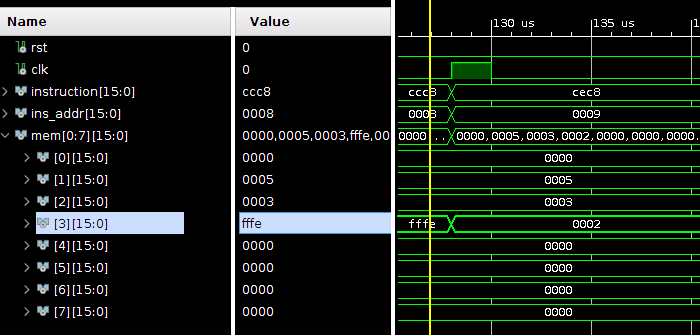
\includegraphics[width=5in]{img/asrinstest.png}
			\caption{Asr instruction simulation}
			\label{fig:asrinstest}
		\end{figure}
		
		\begin{par}
			A simulation of the asr instruction is shown above in Figure \ref{fig:asrinstest}. The instruction performs an arithmetic shift right on register one. The result is stored in register three. In the simulation shown above r1 contains a value of five. After the positive clock edge the asr instruction is executed and two is written to register three. The functionality is verified because the one bit arithmetic shift right of five is two. 
		\end{par}
		\newpage
		
	\subsection{Asl instruction verification}
		\vspace{.5cm}
		\begin{center}
			\begin{tabular}{|c|c|}
				\hline 
				\textbf{Instruction} & \textbf{Machine Code} \\ 
				\hline 
				asl r3, r1 & 1100111011001000 \\ 
				\hline 
			\end{tabular} 
		\end{center}
		
		\begin{figure}[H]
			\centering
			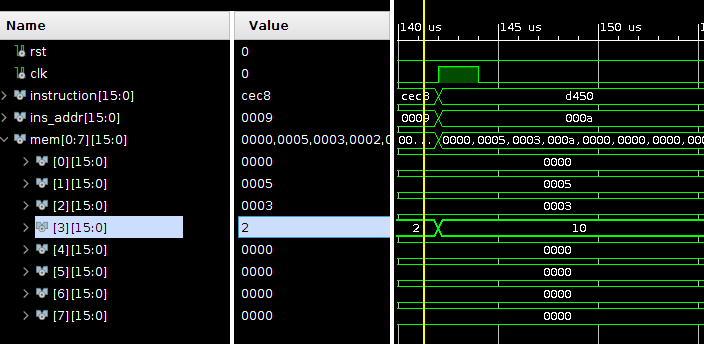
\includegraphics[width=5in]{img/aslinstest.png}
			\caption{Asl instruction simulation}
			\label{fig:aslinstest}
		\end{figure}
		
		\begin{par}
			A simulation of the asl instruction is shown above in Figure \ref{fig:aslinstest}. The instruction performs an arithmetic shift left on register one. The result is stored in register three. In the simulation shown above r1 contains a value of five. After the positive clock edge the asl instruction is executed and ten is written to register three. The functionality is verified because the one bit arithmetic shift left of five is ten. 
		\end{par}
		\newpage
		
	\subsection{Addi instruction verification}
		\vspace{.5cm}
		\begin{center}
			\begin{tabular}{|c|c|}
				\hline 
				\textbf{Instruction} & \textbf{Machine Code} \\ 
				\hline 
				addi r1, 3 & 1101000001000011 \\ 
				\hline 
			\end{tabular} 
		\end{center}
		
		\begin{figure}[H]
			\centering
			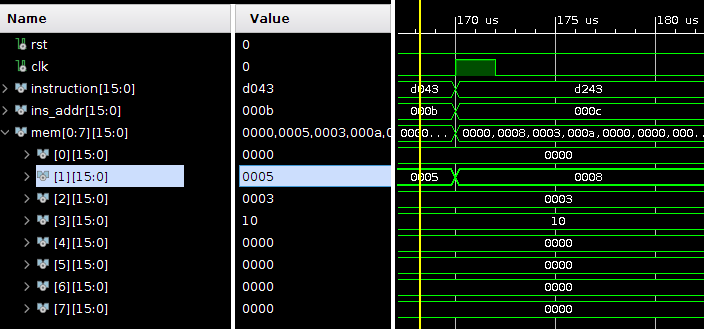
\includegraphics[width=5in]{img/addiinstest.png}
			\caption{Addi instruction simulation}
			\label{fig:addiinstest}
		\end{figure}
		
		\begin{par}
			A simulation of the addi instruction is shown above in Figure \ref{fig:addiinstest}. The instruction adds the specified immediate three to the current value in r1. In the simulation, before the positive clock edge, r1 contains the value five after the clock edge r1 contains eight. Since five plus three is eight the instruction is working correctly. 
		\end{par}
		\newpage

	\subsection{Subi instruction verification}
		\vspace{.5cm}
		\begin{center}
			\begin{tabular}{|c|c|}
				\hline 
				\textbf{Instruction} & \textbf{Machine Code} \\ 
				\hline 
				subi r1, 3 & 1101001001000011 \\ 
				\hline 
			\end{tabular} 
		\end{center}
		
		\begin{figure}[H]
			\centering
			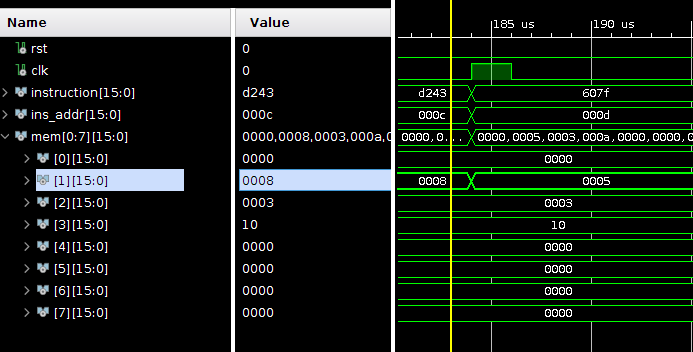
\includegraphics[width=5in]{img/subiinstest.png}
			\caption{Subi instruction simulation}
			\label{fig:subiinstest}
		\end{figure}
		
		\begin{par}
			A simulation of the subi instruction is shown above in Figure \ref{fig:subiinstest}. The instruction subtracts the specified immediate three from the current value in r1. In the simulation, before the positive clock edge, r1 contains the value eight after the clock edge r1 contains five. Since eight minus three is five the instruction is working correctly. 
		\end{par}
		\newpage
		
	\subsection{Lui instruction verification}
		\vspace{.5cm}
		\begin{center}
			\begin{tabular}{|c|c|}
				\hline 
				\textbf{Instruction} & \textbf{Machine Code} \\ 
				\hline 
				lui r1, 63 & 0110000001111111 \\ 
				\hline 
			\end{tabular} 
		\end{center}
		
		\begin{figure}[H]
			\centering
			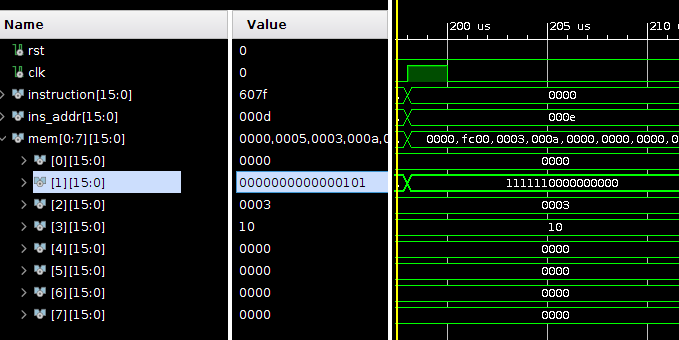
\includegraphics[width=5in]{img/luiinstest.png}
			\caption{Lui instruction simulation}
			\label{fig:luiinstest}
		\end{figure}
		
		\begin{par}
			A simulation of the lui instruction is shown above in Figure \ref{fig:luiinstest}. The Lui instruction loads the upper 6-bits of a register with a specified immediate value. Lui zeros the bottom 10-bits of the specified register. In the simulation the specified immediate value is 63 or binary 111111. After the clock edge it can be seen that lui correctly loaded the 6-bit immediate and cleared the bottom 10-bits of register one. 
		\end{par}
		\newpage
		
\section{ Branching Instruction Testing}
	\subsection{CMP instruction verification}
		\vspace{.5cm}
		\begin{center}
			\begin{tabular}{|c|c|}
				\hline 
				\textbf{Instruction} & \textbf{Machine Code} \\ 
				\hline 
				cmp r0, r0 & 1101010000000000 \\ 
				cmp	r1, r2 & 1101010001010000 \\
				cmp	r2, r1 & 1101010010001000 \\
				\hline 
			\end{tabular} 
		\end{center}
		
		\begin{figure}[H]
			\centering
			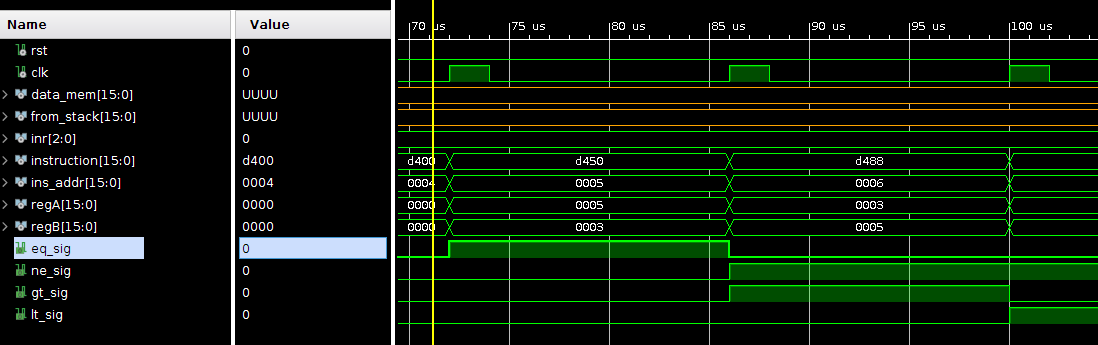
\includegraphics[width=7in]{img/cmpinstb.png}
			\caption{Cmp instruction simulation}
			\label{fig:cmpinstb}
		\end{figure}
		
		\begin{par}
			A simulation of the cmp instruction is shown above in Figure \ref{fig:cmpinstb}. Three cmp instructions are executed showing each possible output of the cmp flags (eq\_sig, ne\_sig, gr\_sig, lt\_sig). The cmp instruction is used before a conditional branch instruction to determine if the branch should be taken. 
		\end{par}
		\newpage
		
	\subsection{Beq instruction verification}
	\vspace{.5cm}
	\begin{center}
		\begin{tabular}{|c|c|}
			\hline 
			\textbf{Instruction} & \textbf{Machine Code} \\ 
			\hline 
			cmp r2, r1 & 1101010010001000 \\ 
			zero r4 & 1100100100100100 \\
			addi r4, 3 & 1101000100000011 \\
			bne		2 & 0010100000000010 \\
			zero	r4 & 1100100100100100 \\
			blt		2 & 0011100000000010 \\
			zero	r4 & 1100100100100100 \\
			zero	r1 & 1100100001001001 \\
			zero	r2 & 1100100010010010 \\
			cmp		r1, r2 & 1101010001010000 \\
			beq		2 & 0010000000000010 \\
			zero	r4 & 1100100100100100 \\
			zero	r1 & 1100100001001001 \\
			zero	r2 & 1100100010010010 \\
			addi	r1, 1 & 1101000001000001 \\
			cmp		r1, r2 & 1101010001010000 \\
			bgt		2 & 0011000000000010 \\
			zero	r4 & 1100100100100100 \\
			hlt & 0000000000000000 \\
			\hline 
		\end{tabular} 
	\end{center}
	
	\begin{figure}[H]
		\centering
		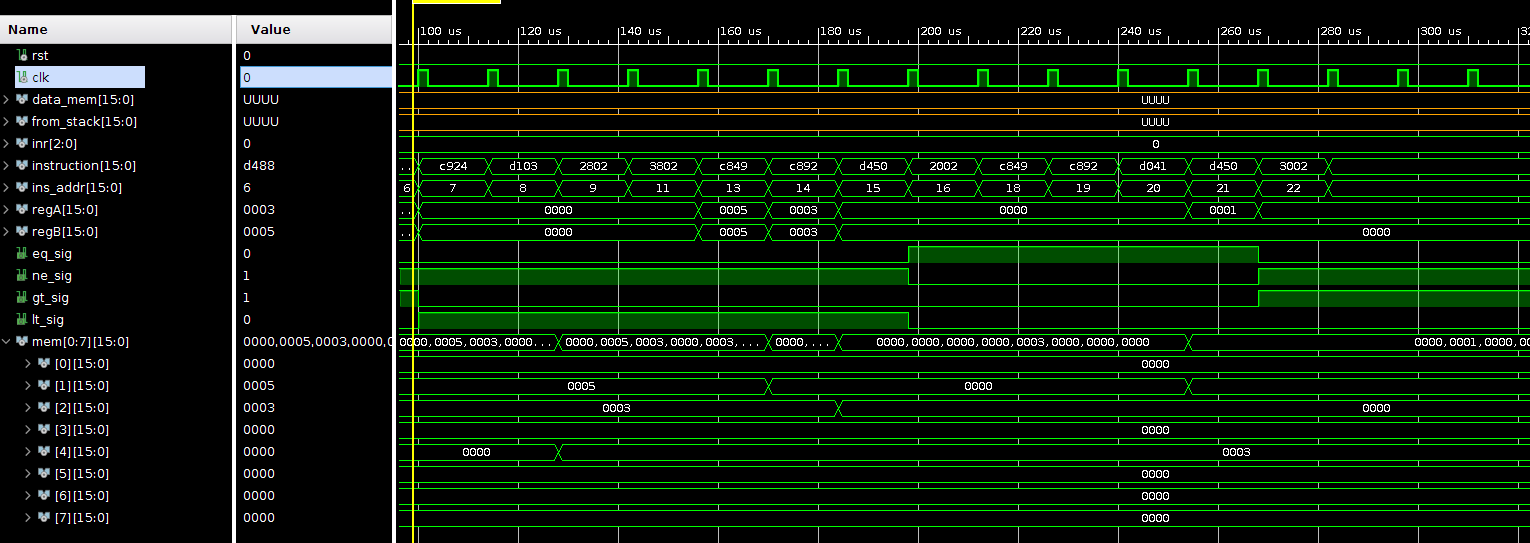
\includegraphics[width=7in]{img/beqinstest.png}
		\caption{Beq instruction simulation}
		\label{fig:beqinstest}
	\end{figure}
	
	\begin{par}
		A simulation of the conditional branching instructions is shown above in Figure \ref{fig:beqinstest}. Each conditional branch instruction is tested. The program gets to the end without clearing the value in r4 this shows that each of the four unique conditional branch instructions worked. In the above code zero is a pseudo-instruction that xors a register with itself. 
	\end{par}
	\newpage
	
	\subsection{Jalr instruction verification}
		\vspace{.5cm}
		\begin{center}
			\begin{tabular}{|c|c|}
				\hline 
				\textbf{Instruction} & \textbf{Machine Code} \\ 
				\hline 
				addi r1, 1 & 1101000001000001 \\ 
				jalr r3, r0 & 1101010001010000 \\
				\hline 
			\end{tabular} 
		\end{center}
		
		\begin{figure}[H]
			\centering
			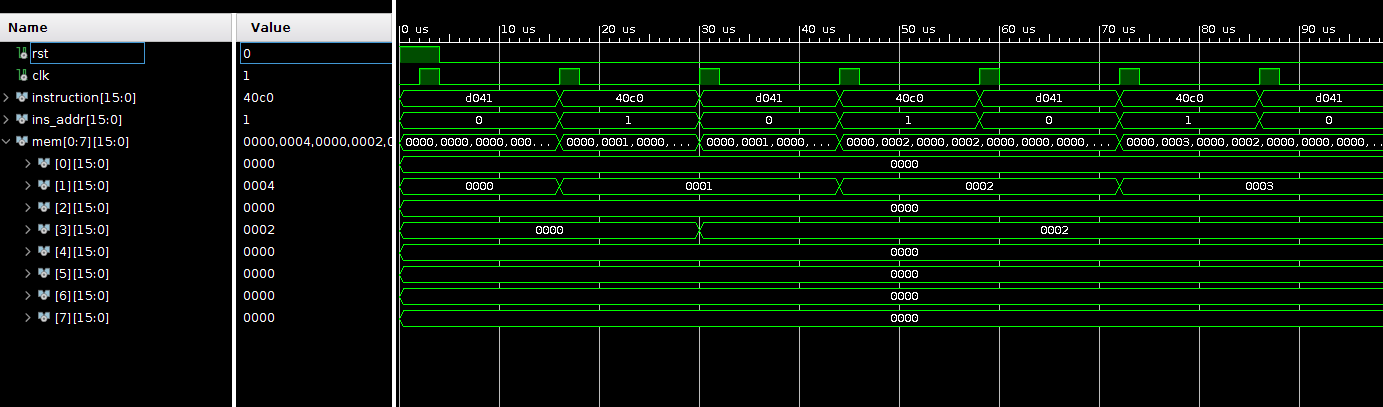
\includegraphics[width=7in]{img/jalrinstest.png}
			\caption{Jalr instruction simulation}
			\label{fig:jalrinstest}
		\end{figure}
		
		\begin{par}
			A simulation of the jalr instruction is shown above in Figure \ref{fig:jalrinstest}. The jump and link register instruction works as indicated by the increasing values of register one. The simulation also shows the correct return address loaded into register three. 
		\end{par}
		\newpage

\section{ CPU Test Program }

	\begin{figure}[H]
		\centering
		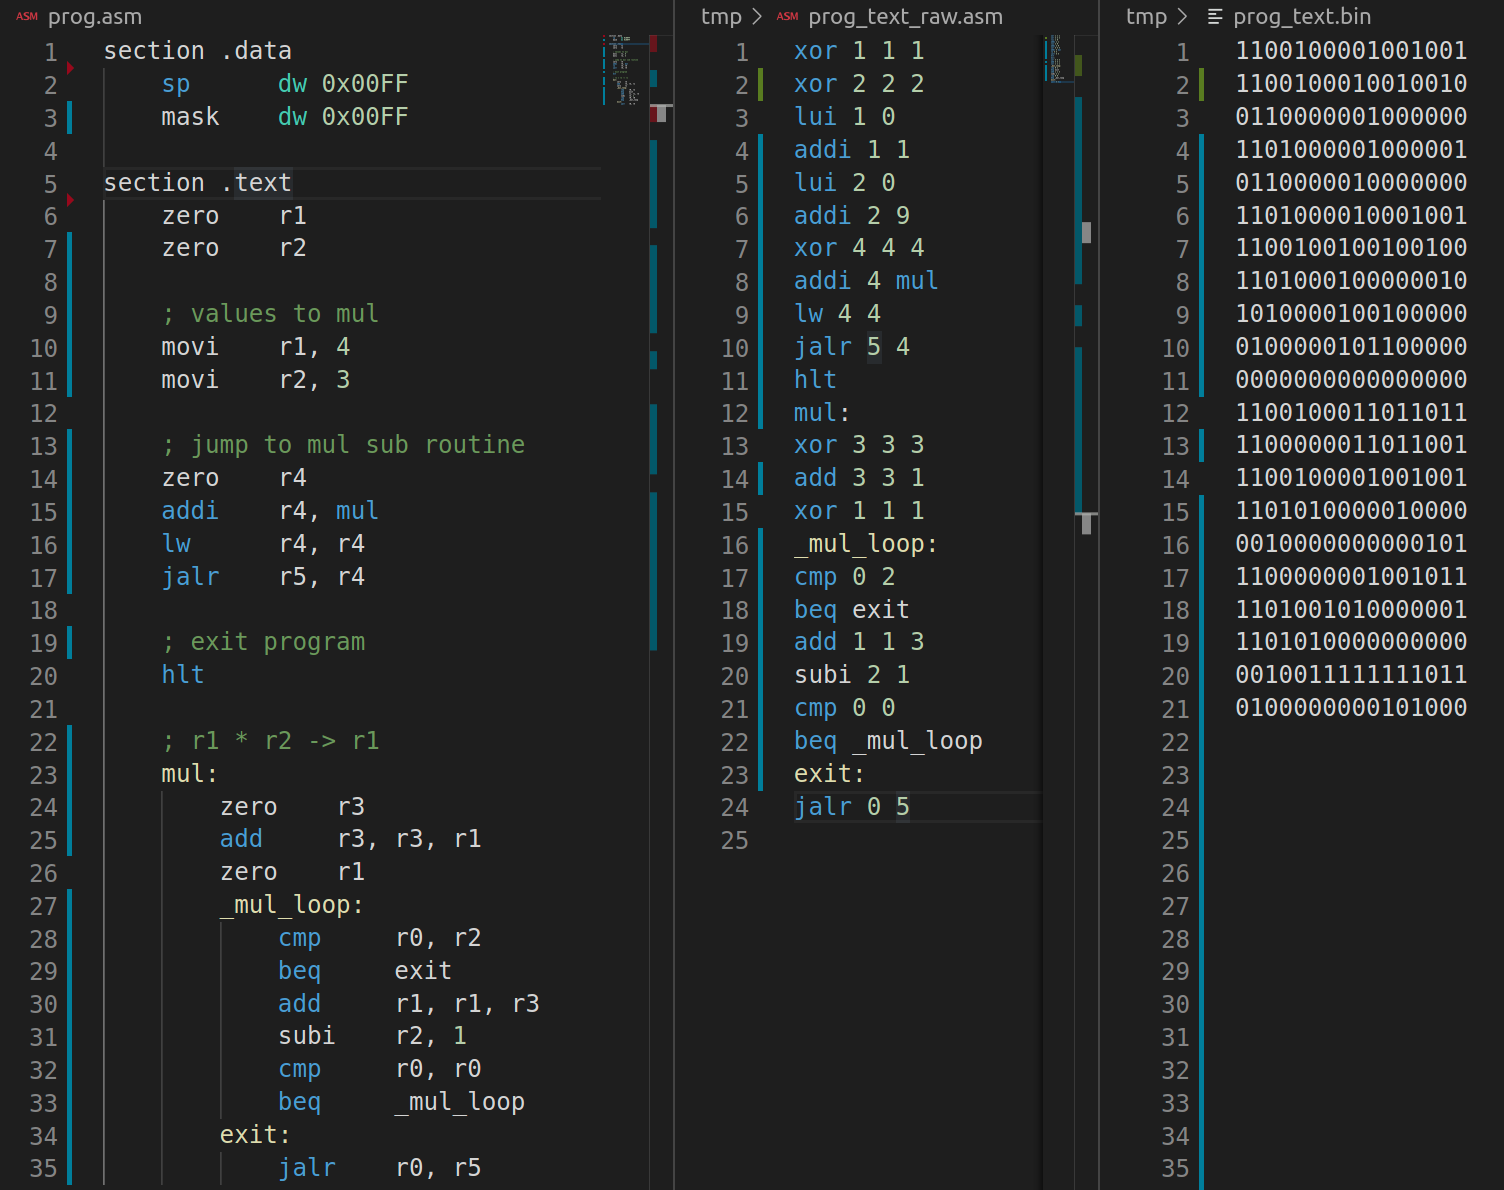
\includegraphics[width=5in]{img/program.png}
		\caption{Software Multiplication Test Program}
		\label{fig:tprog}
	\end{figure}

	A test program is created to further verify the functionality of the Shell CPU. An obvious short coming of the Shell ISA is that it provides no multiplication instruction. To remedy the lack of multiplication hardware support the test program illustrates how multiplication can be performed in software Figure \ref{fig:tprog}. Three code segments can be seen in Figure \ref{fig:tprog}. The first code segment (far left) is the high level assembly code for the program. The middle code segment contains the bare metal assembly code (no pseudo-instructions or register names). The last code segment shows the machine code that is loaded onto the processor to perform the multiplication. It is important to note that this code not only performs multiplication but does so in a reusable way with subroutines.  
	
	\begin{figure}[H]
		\centering
		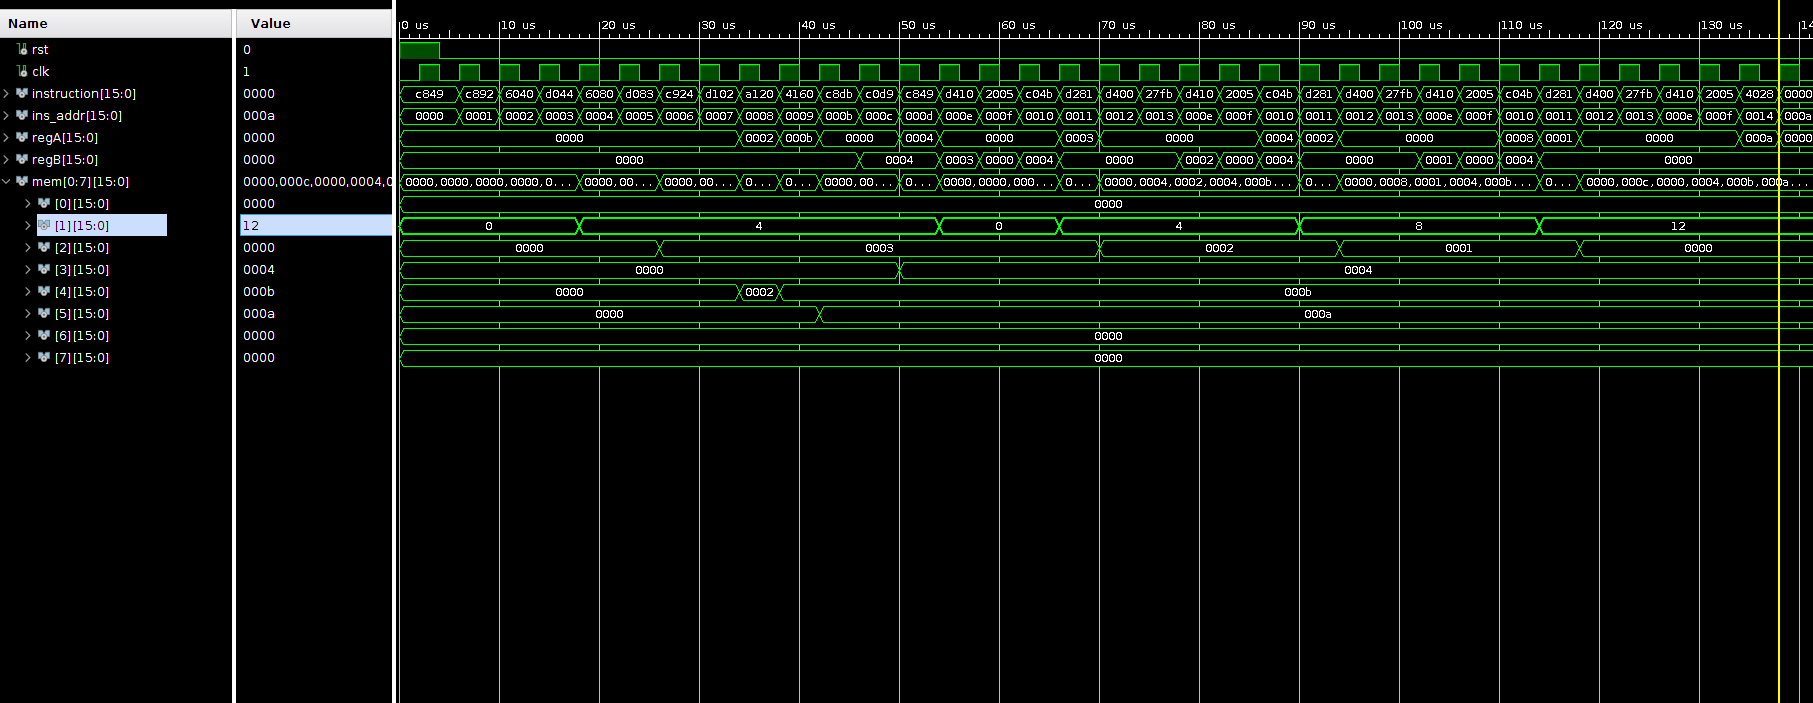
\includegraphics[width=6in]{img/testprogsim.png}
		\caption{Software Multiplication Test Program Simulation}
		\label{fig:tprogsim}
	\end{figure}

	The simulation of the test program from Figure \ref{fig:tprog} can be seen in Figure \ref{fig:tprogsim}. In the test program the values three and four were passed into the multiplication subroutine. The subroutine is expected to compute the result and return to the caller. In the simulation it can be seen that twelve, the answer to three times four, is stored in register one. The program then takes a few clock cycles to return from the multiplication subroutine where it then executes a halt instruction. 

\end{document}